% Figure 12, written by Code/figure_line_ratios.py from results/laptop_timings/timings.csv
\begin{figure}[ht]
    \centering
    \begin{subfigure}[t]{0.48\textwidth}
        \centering
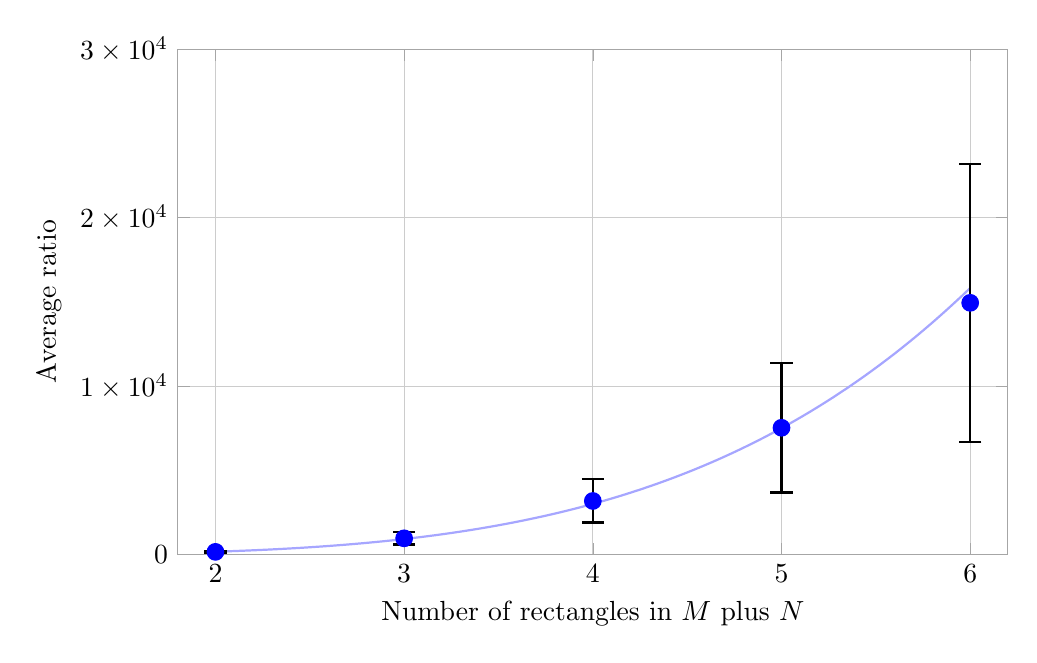
\begin{tikzpicture}
\begin{axis}[
    set layers,
    width=\linewidth,
    height=8cm,
    xmin=1.8,
    xmax=6.2,
    ymin=0,
    ymax=30000,
    xtick={2,3,4,5,6},
    ytick={0,10000,20000,30000},
    yticklabels={0,$1\times10^4$,$2\times10^4$,$3\times10^4$},
    scaled y ticks=false,
    xlabel={Number of rectangles in $M$ plus $N$},
    ylabel={Average ratio},
    grid=both,
    major grid style={gray!40},
    minor grid style={gray!20},
    axis line style={gray!70},
    tick style={gray!70},
]

% Best-fit curve y = 10.40 x^4.09 (least squares on log x, log y of the means)
\addplot[
    thick,
    color=blue!35,
    domain=2:6,
    samples=100
] {10.40*x^4.09};

% Error bars (black): mean +/- one standard deviation
\addplot[
    draw=none,
    mark=none,
    error bars/.cd,
        y dir=both,
        y explicit,
        error bar style={draw=black, thick},
        error mark options={draw=black, thick, rotate=90, mark size=4pt},
] coordinates {
    (2,168) +- (0,49)
    (3,972) +- (0,368)
    (4,3189) +- (0,1283)
    (5,7534) +- (0,3846)
    (6,14951) +- (0,8257)
};

% Blue points: mean over the runs (20, 40, 60, 80, 35 runs)
\addplot[
    only marks,
    mark=*,
    mark size=3pt,
    color=blue,
    on layer=axis foreground,
] coordinates {
    (2,168)
    (3,972)
    (4,3189)
    (5,7534)
    (6,14951)
};

\end{axis}
\end{tikzpicture}

    \caption{ Blue points give the average ratio of all lines computed to those of which are through only critical points, varying the total number of rectangles in two rectangle decomposable persistence modules $M$ and $N$. Shown also in blue is the best fit curve for this ratio, $y=10.4x^{4.09}$. \textcolor{blue}{Error bars are shown +/- one standard deviation.} }
    \label{fig:stats_cl_1}
    \end{subfigure}
    \hfill
    \begin{subfigure}[t]{0.48\textwidth}
        \centering
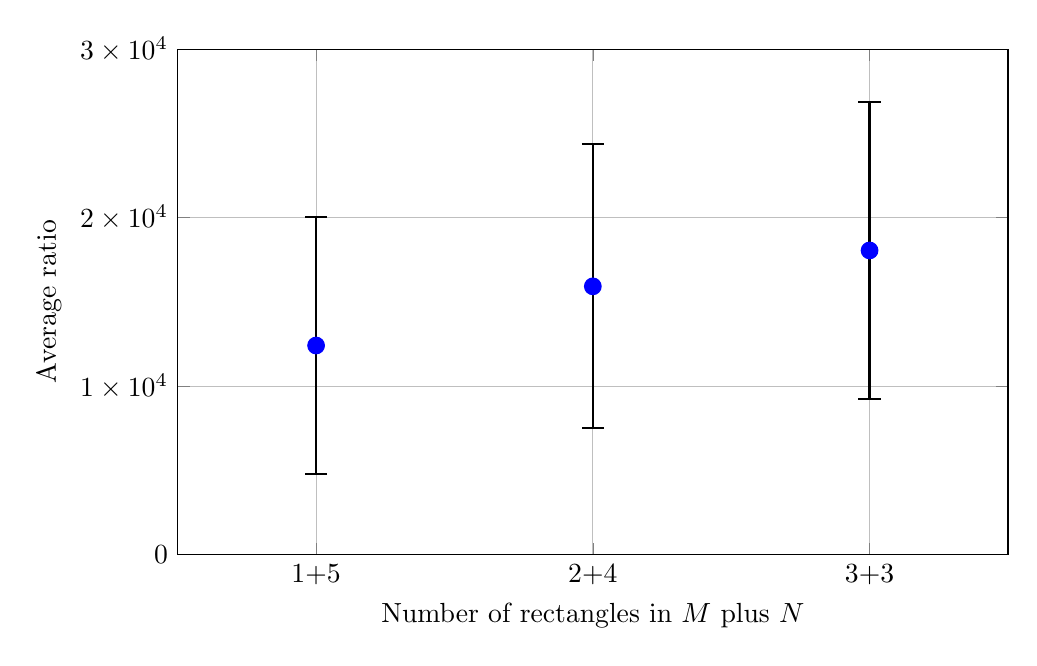
\begin{tikzpicture}
\begin{axis}[
    set layers,
    width=\linewidth,
    height=8cm,
    ymin=0,
    ymax=30000,
    xmin=0.5,
    xmax=3.5,
    xtick={1,2,3},
    xticklabels={1+5,2+4,3+3},
    ytick={0,10000,20000,30000},
    yticklabels={0,$1\times10^4$,$2\times10^4$,$3\times10^4$},
    scaled y ticks=false,
    xlabel={Number of rectangles in $M$ plus $N$},
    ylabel={Average ratio },
    grid=both,
]

% Error bars (black): mean +/- one standard deviation
\addplot[
    draw=none,
    mark=none,
    error bars/.cd,
        y dir=both,
        y explicit,
        error bar style={draw=black, thick},
        error mark options={draw=black, thick, rotate=90, mark size=4pt},
] coordinates {
    (1,12417) +- (0,7623)
    (2,15930) +- (0,8429)
    (3,18060) +- (0,8831)
};

% Blue points: mean over the runs (14, 14, 7 runs)
\addplot[
    only marks,
    mark=*,
    mark size=3pt,
    color=blue,
    on layer=axis foreground,
] coordinates {
    (1,12417)
    (2,15930)
    (3,18060)
};

\end{axis}
\end{tikzpicture}

    \caption{Blue points indicate the average ratio of all lines computed to lines through only critical points for all possible combinations with a total of $6$ rectangles. \textcolor{blue}{Error bars are shown +/- one standard deviation.}}
       \label{fig:stats_cl_2}
    \end{subfigure}
    \caption{Statistics on the ratio between the number of lines through all points (critical and candidate switch points) over the number of lines through only critical points.  }
    \label{fig:stats_cl}
\end{figure}
